% ---------------------------------------------------------------------------- %
% DOCUMENT SETUP
% ---------------------------------------------------------------------------- %
\documentclass[a4paper,11pt,parskip=false, oneside]{scrbook}

\usepackage[utf8]{inputenc}
\usepackage[T1]{fontenc}
\usepackage{lmodern}
\usepackage{amsmath}
\usepackage{amsfonts}
\usepackage{amssymb}
\usepackage{subcaption}
\usepackage{pgfplots}
\usepackage{siunitx}
\usepackage{graphicx}
\usepackage{rotating}
\usepackage{setspace}
\usepackage{changepage}
\usepackage{longtable}
\usepackage{booktabs}
\usepackage{todonotes}
\usepackage{float}

%code formatting in latex:
\usepackage{listings}
\lstset { %
    language=Python,
    basicstyle=\footnotesize,% basic font setting
    numbers=left,
    frame=tb,
}

% tikz pictures and own defined colors
\usepackage{tikz} %loads also xcolor
\definecolor{darkblue}{rgb}{0.047, 0.337, 0.678}
\definecolor{darkgreen}{rgb}{0.13,0.55,0.13}
\definecolor{darkorange}{rgb}{0.93,0.46,0}

% package for setting margins at the sides, top and bottom
\usepackage[left=3cm,right=2cm,top=2.5cm,bottom=2.5cm]{geometry}

% hyperlinks to sections in pdf file
\usepackage[bookmarksnumbered,pdftitle={Master's Thesis},hyperfootnotes=false]{hyperref} 
\hypersetup{colorlinks, citecolor=black, linkcolor=black, urlcolor=black}


% citation style
\bibliographystyle{abbrvdin}

\setcounter{secnumdepth}{1}
\setcounter{tocdepth}{1}

% Some fixes for the warnings
\usepackage{scrhack}
\pgfplotsset{compat=1.16}
\pdfsuppresswarningpagegroup=1

\onehalfspacing

% ---------------------------------------------------------------------------- %
% Blank pages
% ---------------------------------------------------------------------------- %

 \newcommand*{\blankpage}{%
	\vspace*{\fill}
	{\centering This page intentionally left blank.\par}
	\vspace{\fill}}
\makeatletter
\renewcommand*{\cleardoublepage}{\clearpage\if@twoside \ifodd\c@page\else
	\blankpage
	\thispagestyle{empty}
	\newpage
	\if@twocolumn\hbox{}\newpage\fi\fi\fi}
\newcommand\mtd[1]{\textcolor{red}{#1}}

\begin{document}

% ---------------------------------------------------------------------------- %
% TEXT SETUP AND LISTS
% ---------------------------------------------------------------------------- %
% Trennvorschläge
%all words with wrong default hyphenation can be correctly defined here.
\hyphenation{
pro-duc-tion
ef-fort-less
}

% empty page at the beginning (optional)
%\newpage
%\thispagestyle{empty}
%\section*{ }

% Cover page %
\thispagestyle{empty}
\newcommand{\titelseite}[2]{
\begin{tikzpicture}[overlay]
\draw [rounded corners, line width=0.05cm, color=darkblue] (-1.2,-25.8) -- (-1.2,-4) -- (16,-4) -- (16, -24.3);
\node [right] at (-1.2,0) {
\includegraphics[height=1.5cm]{./figures/uni-logo.pdf}};
\node [left] at (16.025,0) {
\includegraphics[height=1.4cm]{./figures/lsbLogo.pdf}};
\draw [fill=darkblue, color=darkblue](-1.2,-25.8) -- (-1.2,-25.5) --(-1.2,-23.8)-- (16.025, -23.8)--(16.025,-25.8);
\node [right, white] at (0,-24.25) {\large{\textsc{#1}}};
\node [right, white] at (0,-25.25) {\large{\textsc{#2}}};
\end{tikzpicture}
}
\newcommand{\titel}[2]{
\begin{center}
\doublespacing
\textcolor{darkblue}{\huge{#1}}\\[1cm]
\textcolor{darkblue}{\Large{\textit{#2}}}\\[3.9cm]
\singlespacing
\end{center}
}

\begin{titlepage}

\titelseite{Master's Thesis}{University of Rostock}

\vspace*{5cm}

\titel{A Data-Processing Framework for \\ Time-Series Operational Vessel Data } {simplify the process of handling marine data}
\vspace{3cm}


\begin{tabular}{p{3.2cm}|p{0.1cm} p{10.5cm}l}
Name: & & Ba Cong Le\\
Student ID: & & 222100012\\
Subject: & & Big data and Marine technology\\
E-Mail: & & cong.ba@uni-rostock.de\\
Supervisors: & & Prof. Dr.-Ing. Stefan Lüdtke\\
 & & Prof. Dr.-Ing. Florian Sprenger\\
Chair: & & Marine Data Science\\ 
& & Ship Design\\
Faculty: & & IEF and MSF\\
Thesis schedule: & & 20 weeks\\
Submission: & & 01.03.2025\\
\end{tabular}
\end{titlepage}

\restoregeometry

\newpage
\thispagestyle{empty} \enlargethispage{20mm} \vspace*{25mm}%
\normalsize
\phantom{x}
\vfill
\noindent Copyright \copyright\ \the\year, Ba Cong Le\\
All rights reserved, text, pictures and graphics are protected
material.
\\[10mm]
Ba Cong Le\\
\makeatletter{cong.ba@uni-rostock.de}\makeatother \\[5mm]
\vspace{10mm} \noindent \scriptsize This document was set with \LaTeX on \today.
\clearpage

% Abstract
\singlespacing
\normalsize
\chapter*{Abstract}\label{chap:abstract}

%\mtd{Here is the abstract: what is the research topic? what is achieved?}

%\begin{abstract}

%This thesis proposes a framework for efficient saving/ modernize/ simplify the process of collecting, formatting, storing, visualize of operational vessel data. 


The proposed thesis focuses on developing a comprehensive data-processing framework tailored for operational vessel time-series data (OVD). As the maritime industry undergoes digitalization, an increasing amount of vessel data is generated from sensors, navigation systems, and operational logs. However, a lack of standardization across different fleet management systems creates challenges in processing, storing, and analyzing this data efficiently. To address these issues, the thesis proposes a scalable, modular framework that can handle large volumes of OVD, ensuring interoperability across various data sources. The framework encompasses data collection, cleaning, storage, and presentation, leveraging InfluxDB database, to manage time-series data. A customizable dashboard interface is also developed to enable data analysis and gain insights. 


Keywords: operational vessel data, marine data science, AIS data, data-processing framework

%\end{abstract}






\newpage
\chapter*{Acknowledgement}\label{chap:ack}
I would like to express my sincere gratitude to MSF, IEF
I am also deeply thankful to my supervisors

% roman page numbering
\pagenumbering{roman}

% Draw Table of Contents
\newpage
\tableofcontents

% Lists in TOC
\addcontentsline{toc}{chapter}{Lists}

% Abbreviations
%\chapter*{List of Abbreviations}
\chapter*{List of Abbreviations}
\addcontentsline{toc}{section}{List of Abbreviations}

\begin{longtable}[c]{>{\bfseries}p{3cm} p{11.9cm}}
	Abbreviation & \textbf{Meaning} \\[3ex]
	\endfirsthead
	Abbreviation & \textbf{Meaning} \\[3ex]
	\endhead
	OVD&Operational vessel data \\[2mm]
	AIS&Automatic identification system\\[2mm]
	DPF&Data-processing framework\\[2mm]
    SQL&DStructured Query Language\\[2mm]
\end{longtable}
%\chapter*{List of Formulas}
\addcontentsline{toc}{section}{List of Formulas}

\begin{longtable}[l]{>{$}p{1.6cm}<{$}>{\centering$}p{1.7cm}<{$}p{4cm}}
	\textbf{Symbol} & \textbf{Unit} & \textbf{Meaning} \\[3ex]
	\endfirsthead
	\textbf{Symbol} & \textbf{Unit} & \textbf{Meaning} \\[3ex]
	\endhead
	\alpha & ^\circ & Angle \\ [2mm]
    x & mm & Coordinate \\ [2mm]
\end{longtable}
\clearpage

%__________________________
% Erklärung zu den longtables:
% \begin{longtable}[l]{>{$}p{1.6cm}<{$} >{\centering$}p{1.7cm}<{$} p{4cm}}
% >{pre} : this command is set before every item in that column
% <{after} : this command is set after every item in that column
% here: pre and after are "$", to make the math modus active in the whole column





% List of Figures
\addcontentsline{toc}{section}{List of Figures}
\listoffigures

% List of Tables
\addcontentsline{toc}{section}{List of Tables}
\listoftables

\clearpage

% ---------------------------------------------------------------------------- %
% MAIN CONTENTS
% ---------------------------------------------------------------------------- %

\onehalfspacing
\pagenumbering{arabic}

% \input{./includes/01_templates}

\chapter{Introduction}\label{chap:Intro}



\section{Background and Motivation}
% \mtd{1 page in total \\}
% \mtd{1 para to describe what is the current situation: how is the intersection between marine industry and digitization, the state of marine data management. (big picture) \\
% 2 para what is the short coming, imperfect things, challenges related to data collection, storage, and analysis in marine operations. \\
% - 1 para about frameworks in maritime.\\
% - 1 para identify any gaps or inefficiencies in current systems that your work aims to address.\\
% 1 para what is your solution to fill in the gaps\\
% }

Advances in shipbuilding, engine technology and navigation over the centuries have expanded global trade, making maritime transport indispensable. 
%This is driven by the increasing global demand for shipping worldwide and the requirement of cost optimization and reducing footprint. 
In recent decades, digitization has emerged as a key development in marine shipping, reshaping the maritime industry to meet the growing volume of goods, the need for cost-efficient operations and the demand for reducing environmental impact.
Nowadays, many decisions in marine industry are driven by data analytics from on-board data, which has proved the value of digitizing ship.
Maersk Line, for example, has installed IoT sensors on its 600 vessels for fuel economy enhancement, voyage optimization, container monitoring and empty container optimization. \cite{raza_digital_2023}. 
%As volume of goods and vessels rises, efficient and cost-effectiveness operations but reducing environmental impact are now more critical than ever.

The intelligent use of operational data of vessels plays a crucial role in transforming future maritime services.
Operational data within the maritime sector is vast and varied, sourced from a multitude of
sensors, cameras, radar, GPS, via digital communication technologies like analog signal, Ethernet, Wi-Fi and Bluetooth.
As a result, the volume of global ship data has grown exponentially, reaching the scale of "big data,", but with limited standards.
For instance, AIS data, a global standard for vessel tracking, is mandatory for ships over 2 tons.
According to a study, MarineTraffic.com collected around 30 GB of AIS data daily in 2013, and this figure constantly increasing \cite{webdigitship}. 
When OVD is effectively handled, any ship could serve as a mobile observation platform and provide a lot of valuable information for research in fields such as shipbuilding, meteorology and more.  


Despite the potential of such data, the maritime industry faces a significant challenge: lack of universally shared standard for operational data across the marine transportation ecosystem, such as among fleet management systems. This is partly due to concerns about data privacy and lack of interoperability between different IT systems involved in the field of maritime logistics. Without a transparent data-processing framework shared among ship owners, the integration of operational vessel data sources will therefore take practitioners and researchers time and effort in data science tasks. 

To address this challenge, this thesis introduces a data-processing framework for operational vessel data that can assimilate data from various data providers. 
The framework, attached with its software, is designed to automatically acquire, clean and consolidate the data, which may exist in heterogeneous sources (e.g., files, XML, JSON, databases), and in different locations. It ensures that data from different locations and formats can be stored in a common database for a wide range of later analysis purposes. The proposed framework is expected to be able to automatically handle large volume of OVD from many vessels.
Additionally, the framework is designed to be easy to understand, because it is based on well-established data science workflows. 
\section{Problem statement}
%\mtd{Define the specific problem your thesis is addressing. State the core problem and including problems regarding marine data processing.}
%The proposed framework is designed to clarify and automate the process of working with  operational vessel data,  starting from data collection to data visualization. 
Throughout a ship’s journey, operational vessel data plays a vital role in monitoring, managing, and optimizing vessel performance.
The OVD, which this thesis deals with, is generated on board using a combination of low-, middle- and high-frequency sampling rates, using both automatic and manual methods. This results in complex, large-scale, and heterogeneous data, characterized by its time-series nature.

In addition, OVD usually contains noisy, incomplete, or redundant information.
\mtd{in construction...}

\section{Objective and Contributions}
%\mtd{Clarify the goals of your research and what it contributes to the field.}
This thesis project is aim at designing and implementing a data-processing framework which can handle time-series operational vessel data.
In the context of this thesis, the data-processing framework consists of a structural approach and a software system designed to efficiently manage, process, and analyze large volumes of data, enable the automation, and scaling data processing tasks.
More specifically, the proposed data processing framework is capable of addressing the challenges in OVD processing by providing a complete and automated solution for all the four stages from data collection, data cleaning, data storage to data presentation.
Furthermore, another objective is to conduct a comprehensive investigation into OVD datasets, in result, a database schema for OVD is developed, including common fields across different OVD datasets.


One use case for the solution presented in its application in formalizing workflows involving OVD in maritime companies, particularly in data analysis scenarios. 
Furthermore, maritime companies can apply the framework to simplify their internal processes of monitoring and optimizing fleet performance. 
%or identifying patterns might go unnoticed in the report data.
In general, the framework can accelerate the process of transforming raw data into meaningful insights. Researchers and analysts can utilize the framework to rapidly assess shipping operations across different metrics. 
%\mtd{this para will be complete until 30.12.2024}

\section{Outline}
%\mtd{Briefly summarize each chapter to give the reader an overview of the document.}

The rest of this document follows this structure: Section 2 outlines the related work. Section 3 describes the scope of this research and the requirements for the proposed solution. The design of the data-processing framework is presented in Section 4, supplemented with implementation. Section 5 discusses the results and evaluation. Finally, Section 6 concludes and further development.
\chapter{Related work}\label{chap:relatedwork}

%\mtd{Here is the intro to the thesis context}

The thesis presents in this section what is in background of the research topic of processing time-series OVD. Section 2.1 provides an introduction of operational vessel data, while section 2.2 give out its recent applications. 
%Section 2.3 shows techniques to process OVD that people using to treat this data type.

\section{Operational Vessel Data}

Operational vessel data includes a rich variety of information collected during ship functioning. This data encompasses a wide range of metrics, from navigation details such as speed, heading, and position, to engine performance, fuel consumption, cargo weight, and weather conditions. It also includes data about .... 

Data that is collected from vessel's operation, varies in collecting technology (radar, satellite, sensors), standards, saving formats. From our perspective, most fields in operational vessel data can be categorized into the following three groups:

\begin{itemize}
    \item \textbf{Sensor-based data}: is a combination of both low frequency, middle frequency data come from on-board sensors.
        \begin{itemize}
        \item low frequency: collected every 4 hours, this data is primarily used to report the current state of the vessel, such as performance, which is useful for high-level supervisors.
        \item middle frequency: collected every 15 minutes, this data helps engineers continuously track the efficiency of ship operations, and drives decisions.
        \item high frequency: collected every a second, is the data used to monitor critical components (such as engine's operational status). It allows for instant response to potential issues and provides predictive maintenance.
        \end{itemize}
    \item \textbf{Navigation data}: is managed by automatic identification system (AIS) is an automatic tracking system that contributes to the safety and continuous of marine traffic. AIS is a critical component so it is employed in majority of ships. There are two classes of AIS:
        \begin{itemize}
        \item class A: used by larger commercial vessels. Frequency: every 2 seconds to 3 minutes. 
        \item class B: used by smaller vessels, including pleasure boats. Frequency: every 30 seconds to 3 minutes, depending on the system configuration.
        \end{itemize}
    \item \textbf{Noon report data}: is low-frequency data, it is manually sampled daily or before departure and after arrival, with uncertainty from logger.
\end{itemize}
        
It is true that the amount of OVD is generated is huge and complex. In a cargo ship, there are 400 sensors installed on board. It is often saved on board and retrieved when the ship comes to shore or the real-time data will be send to offshore management via satelite internet.
%Storing these complex information in a common database is a really challenge. To mitigate this tricky problem, the thesis proposed a  schema for operational vessel database to save these non-structured time-series data, the proposed schema and used database engine will be talk further in Design section.


%\section{Storage of marine data}
%\mtd{where is the data stored? how is the data stored? what does the data consist of (data structure)?}

\section{Applications of OVD}
\mtd{current state of the art in vessel data applications?}
\mtd{what current motivations for your system requirements?}

There are many existing applications on OVD in maritime industry. For example, live vessel map is a notable one \cite{liu_visualization_2021}, which leverages AIS data for vessel map analysis or vessel trajectory analysis.  Geometric algorithms are also used to enhance early collision predicting and assess the safety at a sailling area based on navigation data.
Framework for Abnormal Vessel Trajectory Detection, as an example, are capable of detecting irregular vessel movements, which can indicate illegal fishing activities, or potential smuggling operations \cite{sidibe_big_2018}. Analysis for Ship Efficiency \cite{aldous_ship_nodate} uses , Framework for New  Vessel Design \cite{sullivan_prospective_2019} shows the effective of .

In addition, there are several commercial frameworks used by by sailor crew and fleet managers to embrace OVD for real-time decision-support, maintenance advisor and others. 
Complex systems, to name but a few Kongsberg K-IMS, integrated information points on ship to visualize onboard and onshore offices. 
Marine Traffic, FleetMon, and VesselFinder are well-established third-party platforms, having their own framework to aggregate AIS data from multiple sources (both terrestrial and satellite) and provide real-time surveillance services of maritime traffic shipping companies, researchers, and the general public.


In recent years, Marine IoT starts gaining attention from communities. For example, Architectures such as Fog Computing and Edge Computing are applied for accelerate IoT field on smart ship. 
To name, Traxens is an active company providing smart container fleet management, allowing tracking containers' location, status, and condition in real time.

  \mtd{why it motivates your requirement?}
%Additionally, Big data processing frameworks are \cite{wang_big_2018}...

%Despite these advances, there is limited research investing a practical processing framework for operational vessel data. This gap provides an opportunity for this thesis to propose a novel framework that emphasizes on customization and simplicity. The proposed framework can be integrated into internal workflow of companies and allows fleet data holders to easily ingest their data due to a common schema. This ensures greater interoperability and more efficient data processing.

%\section{Data processing in OVD}
%\mtd{current state of the art in data-processing OVD?}


%To the best of our knowledge, none of the existing work on WSN–MCC integration considers the data traffic monitoring, filtering, prediction, compression, and encryption of sensory data before transmitting to the cloud. Our work is the first to consider all these tasks.

\section{ Data-processing frameworks}
\mtd{existing framework for OVD}

There are two common data processing approaches: batch processing and stream processing. The batch processing approach is
efficient in processing high volumes of data collected from time to time. On the other hand,
the stream processing approach performs data processing with a small window of recent
data at one time. This approach can be real-time or near-real-time when there are delays
between the time of transaction and changes are propagated






\chapter{Scope of Research and Requirements} \label{chap:scope}


\section{Scope of Research}
This research concerns with exploring the concept and developing a data-processing framework specifically tailored for maritime operational time-series data.
For a thesis project, some aspects and sub-topics are chosen from list to dive in depth as below:
\begin{itemize}
    \item \textbf{A Modular and Scalable Data-processing Framework} \\
     Ensuring the designed framework is modular, capable of scaling out for different vessel types, operational complexities.
    \item \textbf{Research a Database Schema for OVD} \\
    A comprehensive investigation on storing static and operational vessels data in a unified SQL database, tailored to handle the time-series nature of the data.
    \item \textbf{Interactive Dashboards} \\
    Web-based dashboards that allow analysts to explore and find insights in historical vessels data through an intuitive interface.
    \item \textbf{Run on-premise but cloud-ready} \\
    The framework should be prepared to be deployed on cloud with little hardship in case of big data processing.
\end{itemize} 

\section{Limitations of Research}
To focus on research targets, certain aspects and sub-topics will not be delved into, which we will discuss them in Future Work section of this thesis.
Followings are the research's limitations:
\begin{itemize}
    \item \textbf{Lower-layer solutions } 
    The thesis will not cover technical details how on-board data is transmitted and encoded/decoded by stations, fleet companies. The work of the thesis belongs to a high layer in the ecosystem.
    \item \textbf{Geographical coverage} 
    Operational maritime data available for this thesis is limited and biased to specific geographical regions, vessels, where operational data has been archived and open for access. 
    %The study will focus on these subjects, and findings may not be directly applicable to areas outside this scope.
    %\item \textbf{Dashboard is specific} The purpose of each analysis varies. So my dashboard serves only specific stakeholders. For other specific analysis, people can create their own customized dashboards.
    \item \textbf{Big data} Handling time-series big data from thousands vessels may require cluster computing and distributed system.
\end{itemize} 

\section{Requirements}

\mtd{where does the requirement come from?}
\mtd{requirement for the whole big project? write more big?}
To specify what the thesis implement, this section lists technical and functional requirements of the software which is developed for the framework. The requirements is collected after considering aspects from perspectives of researchers, data analytics, and data engineer in the fields of computer science and ship design \mtd{improve}.
\subsection{Functional requirements}

Functional requirement defines features of the software built for the framework. 
This software contains five main components: data collector, data cleanser, data integrator, data computer and data presenter. The functional requirements for each component are outlined below:
\mtd{improve}
%it means that these features will be designed and implemented in the thesis work.
\begin{itemize}
    \item {Data Collector component}:
     gathers OVD periodically from various sources (eg,. databases, cloud services, data stream) and finally save them to the hard disk under CSV format.
     \item {Data Cleaner component}: 
     enable users to convert raw and noisy AIS data, engine data, fuel consumption data... into clean data according to their cleaning procedures.
     \item Data Integrator component:
    integrates multiple cleaned datasets into a database with a unified schema, free from duplications or inconsistencies.
     \item Data Computer component: this component transforms, enriches and normalizes cleaned data into valuable information. In addition, the cleaned data will also be used for training predictive models. 
     \item Data Presenter component: consists of interactive dashboards facilitating data analysis (eg., filter data by sailing area, seasons, navigational status, filter data, select specific metrics). In terms of visualization, dashboards have to show information in a intuitive way and well-organized. 
%     \item{Component should be encapsulated in containers, which eases deployment and scaling up.}
\end{itemize} 
\subsection{Nonfunctional requirements}

The software, which is implemented in this thesis, is expected to meet the following qualities:
\begin{itemize}
     \item {Encapsulation}: each components (data collector, data cleaner, data integrator, data computer, and data presenter) must be encapsulated and containerized using Docker, ensuring deployment across different environments, including potential cloud platforms.
     \item {Re-usability}: The software provides reusable exemplary scripts that can be easily adjusted for user's specific business and research applications. For example, the data collecting/cleaning script can be reused for a new data source with a few adjustment.
     \item {Extendablility:} 
     The software can be easily customized, allowing the developer to extend or modify, for example adding new fields to the database schema when an external dataset needs to be ingested.
     %\item {Performance}: comparing between InfluxDB and TimescaleDB for the use case of OVD
\end{itemize} 





\chapter{Design \& Implementation} \label{chap:design}


This chapter introduces the concept of the data-processing framework for OVD (Section 4.1). 
Section 4.2 proposes a software, which is designed for this framework.
The rest described the individual modules within the proposed framework in details (Section 4.3, 4.4, 4.5, 4.6).

This chapter present the design and implementation for our OVD software project.
Section \ref{chap:design:overview} provides an overview for the software design, which comprises of separated modules.
These modules will be explained further in the subsequent sections.
Finally, we introduce a setup based on the framework to demonstrate a complete workflow in Section \ref{chap:design:software} \mtd{improve}
% The rest described the individual modules within the proposed framework in details (Section 4.3, 4.4, 4.5, 4.6).


\section{Framework Overview}\label{chap:design:overview}
The framework is designed to be self-contained, easy to utilize and maintain, yet capable of being scaled out to sorts of OVD.
To achieve these goal, we decide to split the software logic into modules, each is isolated in compartment, or \textit{module}.
These modules are self-contained, stand-alone software programs that run on any POSIX environment (Linux, macOS).
A single module is responsible for a stage in the OVD data process: making raw data available, cleaning data from abnormal values, storing in  centralized database in a pre-defined format, as well as extracting meaningful data using scientific methods.
To ensure portability and scalability, we decide to package the modules in software container using Docker along with a Docker-compose script for quick deployment.
However, for horizontal scale up, these independent containers can be deployed in a Kubernetes cluster \mtd{improve}.


% The data-processing framework is designed to handle large-scale, time-series operational vessel data (OVD), facilitating the transformation of raw data into presented insights.
The proposed framework (Figure \ref{fig:design:framework-overview}) composes of four modules, corresponding to four common stages in data engineering: data collection, data cleaning, data storage, data presentation. 
By decoupling the logics, the framework can be extended by adding new module in between existing modules. 
Additionally, the processing capacity of each stage can be scaled by running many containers simultaneously with the same logic scripts \mtd{improve this}.
For management and interaction purpose, each module is provided with a user interface (called "Module management").

\begin{figure}[H]
    \centering
    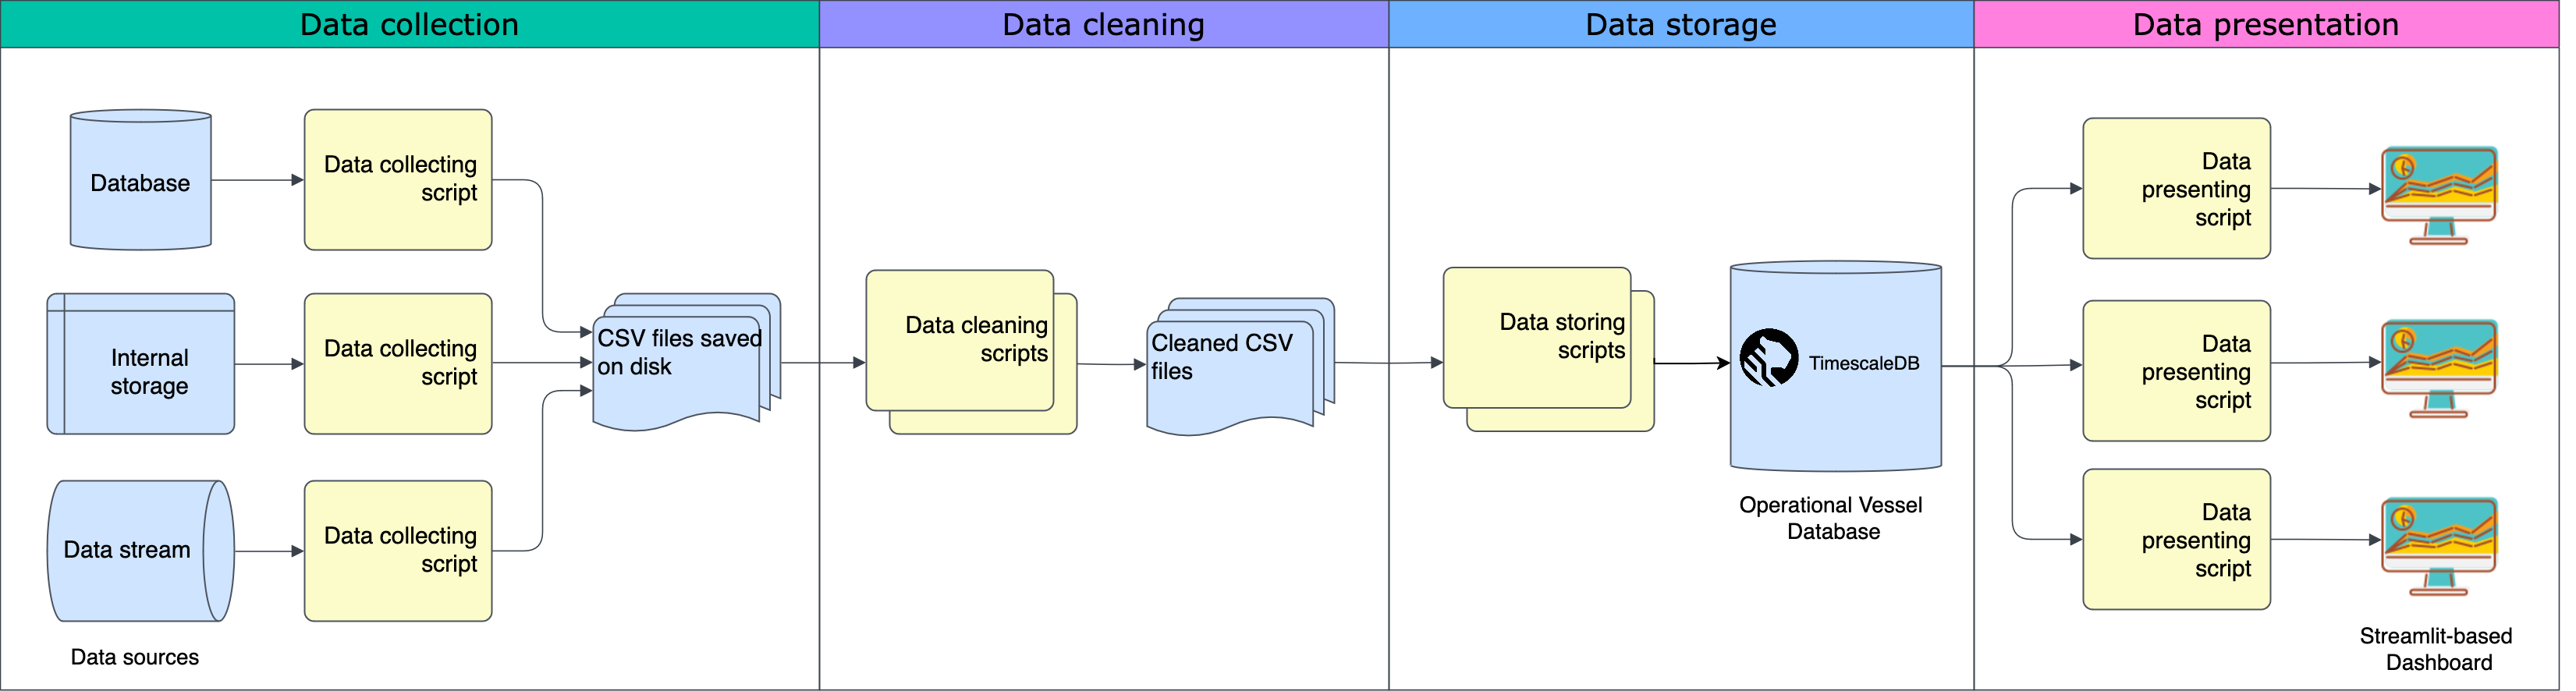
\includegraphics[width=1.0\linewidth]{studentWorkTemplate_en/figures/mt-222100012-framework-overview.drawio.png}
    \caption{The proposed framework for OVD}
    \label{fig:design:framework-overview}
\end{figure}

Starting from the left of Figure \ref{fig:design:framework-overview}, the data collection module is tasked with collecting data automatically from various user-defined data sources. By running collecting scripts periodically, every data sources are saved to the hard disk under CSV format. 
Subsequently, the cleaning module allows user to choose a CSV file on disk and a suitable cleaning script. Then, the module run the cleaning script, which clean the data file and return the cleaned data file to the hard disk (also under CSV format). 
Similarly, the data storage module once again run the selected storing script on the selected cleaned data file to save it to TimescaleDB for long term uses. 
At the last module, the data from TimescaleDB database will be retrieved and computed by dashboards, which ensure the visualization is intuitive and interactive to users.


\begin{figure}[H]
    \centering
    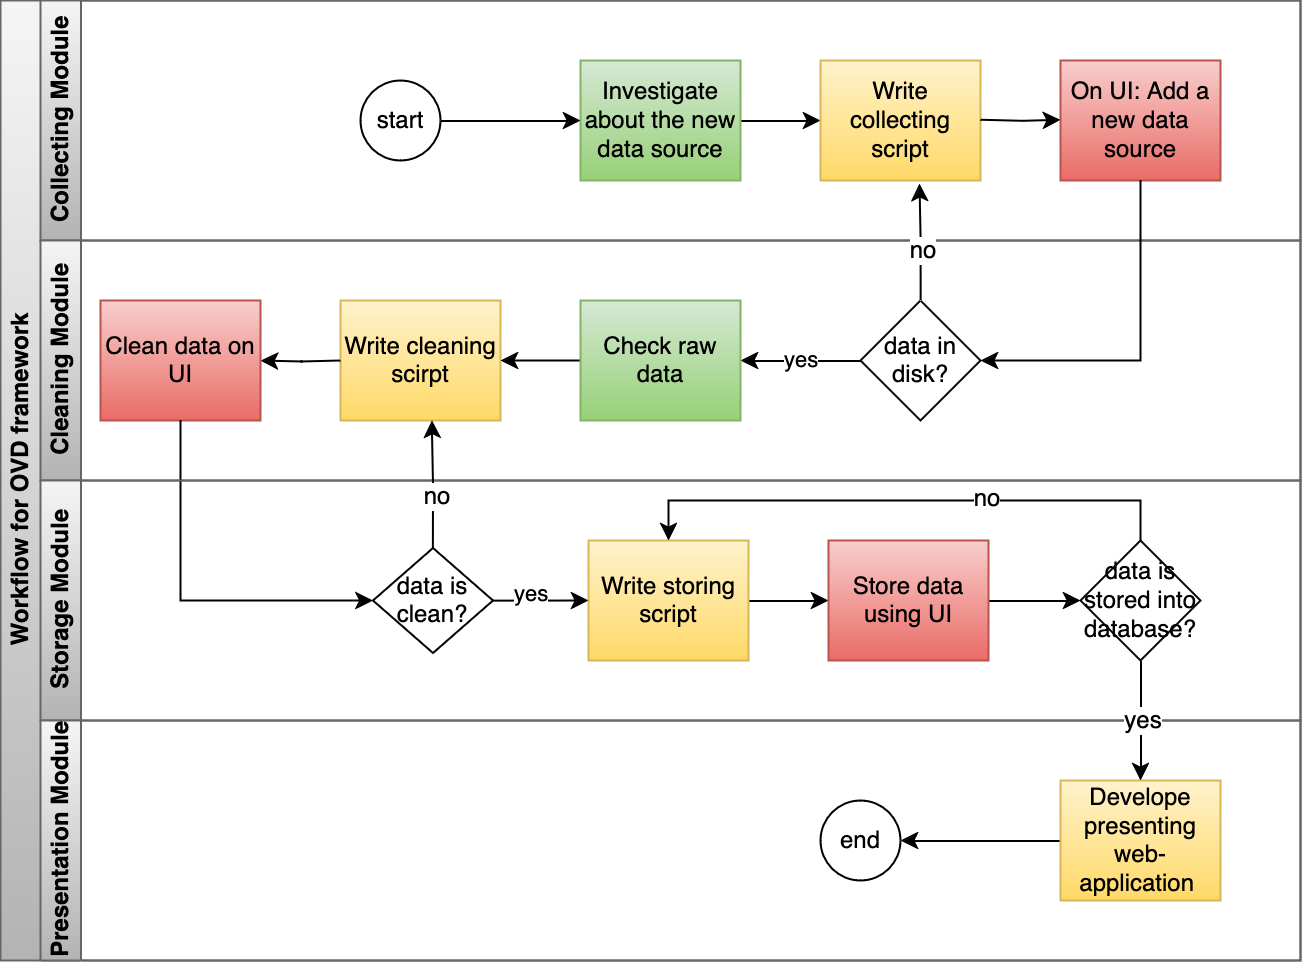
\includegraphics[width=0.8\linewidth]{studentWorkTemplate_en/figures/mt-222100012-workflow.drawio.png}
    \caption{Workflow for user}
    \label{fig:framework-workflow}
\end{figure}

To view the framework from user perspective, Figure \ref{fig:framework-workflow} presents step-by-step workflow. 

\section{Implementation overview}
\label{chap:design:software}
Along with the proposed framework, we implemented a software to manage and conduct works on the framework more efficiently. 
The framework software is implemented in Python programming language, and can be run on different operating systems. The software is also split to four modules corresponding to four modules of the data-processing framework: data collecting module, data cleaning module, data storage module and data presentation module. Each module has "Module Management" component and Backend component (i.e., data collector, cleaner, integrator, computer). "Module Management" components are a Streamlit-based website, allow user to work with these module. The logic of each module is located at its Backend component.
There are data sharings among modules, which creates the mutual communication and continuity between modules. To facilitate the technical requirement, Docker container and Docker volume are employed to this software. 
The whole system architecture is depicted in Figure \ref{fig:software-architecture}


\begin{figure}[H]
    \centering
    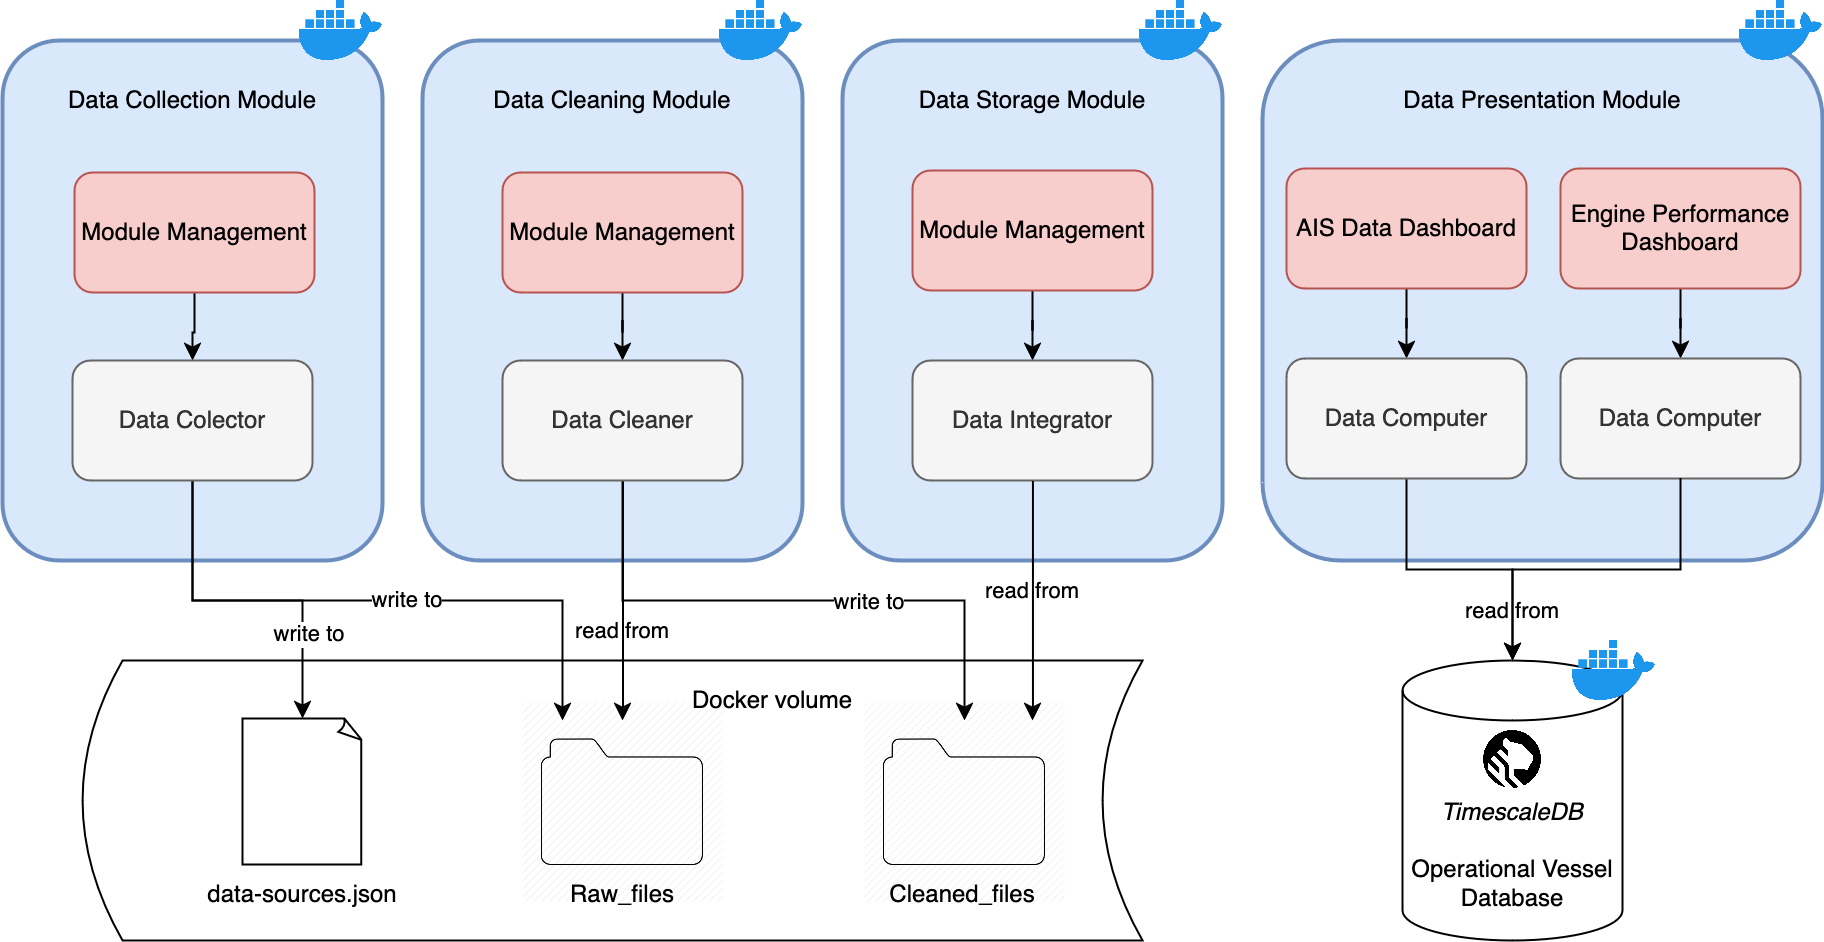
\includegraphics[width=1.0\linewidth]{studentWorkTemplate_en/figures/mt-222100012-system-architecture.drawio.png}
    \caption{Docker deployment}
    \label{fig:software-architecture}
\end{figure}

\mtd{1 para why you choose Docker container? why you choose Docker volume?}
Setting up with Docker, the software utilizes the portable and stable characteristics of Docker, help it deploy more easily. Docker Volume is used to keep up-to-dated of code and data files across the four Docker containers. 
The database, which is used for this framework is TimescaleDB, is also containerized and be access via TCP protocol. 

\mtd{Screenshot of one of four "Module Management" }


\section{Module 1: Data collection}
\mtd{write down here objectives of data collection module}

\subsection{Overview}
The primary goal is to gather raw data from various sources (databases, APIs, etc.) in a convenient and flexible manner. Additionally, the captured data should be comprehensive, complete to support downstream processing.
From the UI, user can monitor the amount of raw data 

At first, the data collection module saves information about data sources given by user to data-sources.json. 
For user, the module's frontend enables add, delete and edit a data source. Meanwhile in the backend, the data collector accesses data source periodically, download data and convert to CSV format, saved to the local disk.

\subsection{Workflow}
\mtd{ghi ro rang: nguoi dung cung cap script, chon url, chon cho luu, thiet lay chay lap lai may ngay mot lan, ...}

\subsection{Software Implementation}
\mtd{API server, Python runner, Streamlit, ...}

\subsection{Deployment}
\mtd{Yeu cau: port mo, docker volume, stateless for scaling. Module nay noi chuiyne voi cac modulke khac nhu the nao, voi nguoi dung nhu the nao (web, cmd line, api, ...)}
\mtd{du lieu luu o dau (path) trong container, va ben nguoi host, permission for data to access from host}

\subsection{Saving data sources}
\mtd{move to implementation}
Each data source is saved with attributes

\begin{longtable}{|c|p{4cm}|p{8cm}|}
    \hline
    \textbf{Index} & \textbf{Attribute} & \textbf{Description} \\ \hline
    \endfirsthead
    \multicolumn{3}{c}%
    {{\bfseries Table continued from previous page}} \\
    \hline
    \textbf{Index} & \textbf{Attribute} & \textbf{Description} \\ \hline
    \endhead
    \hline \multicolumn{3}{|c|}{{Continued on next page}} \\ \hline
    \endfoot
    \hline
    \endlastfoot

    1 & Source Name & The name of the data source or system providing the data. \\ \hline
    2 & Source URL & The URL or endpoint where the data can be accessed. \\ \hline
    3 & Source Description & A brief description of the data source and what kind of data it provides. \\ \hline
    4 & File Format & The format in which the data is provided or stored (e.g., CSV, JSON). \\ \hline
    5 & Collecting Script & The script or method used to collect the data (e.g., Python script, API call). \\ \hline
    6 & Category & The category of the data source (e.g., sensor data, weather data). \\ \hline
    7 & Collecting Frequency & The frequency at which the collecting script is scheduled to run by the system (Every minute, Hourly, Dayly, Weekly, Monthly). \\ \hline

\end{longtable}
This is an example of 2 data sources saved json file:

\begin{verbatim}
[
    {
        "name": "[AIS Hub] csv",
        "url": "sdf",
        "description": "sdfsdfsdf"
    }
]
\end{verbatim}

\section{Module 2: Data cleaning}
\subsection{Overview}
\mtd{write down here objectives of this data cleaning module}
This module allows user to choose the data file and its cleaning scripts to clean processing.
With one script, one cleaning procedures but can reused for different file. It will reduce time for this cleaning task.

\subsection{Eliminate common errors in OVD}
This is some common errors occurred in OVD.


\begin{table}[]
\begin{tabular}{|l|l|l|}
\hline
\textbf{Category} & \textbf{Error} & \textbf{Example} \\ \hline
Column-related errors & wrong column names & abcd \\ \hline
 & wrong column data type &  dbe \\ \hline
 & wrong column data format & xyz \\ \hline
 &  &  \\ \hline
Row-related errors & missing row & \begin{tabular}[c]{@{}l@{}}Depends on the requirements: \\ ignore, or mark for post processing\end{tabular} \\ \hline
 & duplicated row & Detect duplication and remove on needed \\ \hline
 & consecutive rows are inconsistent & Detect by comparison and -remove/edit \\ \hline
 &  &  \\ \hline
\begin{tabular}[c]{@{}l@{}}Corrupted\\ cell's content\end{tabular} & NaN, null, Unknown values & Depends on requirements: remove rows, or mark. \\ \hline
 & miss-typed values & Replace with the correct values or remove that row \\ \hline
 & outlier values: too high, to low values & Remove that row \\ \hline
 & wrong timestamp & Remove that row \\ \hline
 &  &  \\ \hline
\end{tabular}
\end{table}


\subsubsection{Error 1.1}

\subsubsection{Error 1.2}

\section{Module 3: Data storage}
\subsection{Overview}

\subsection{Database schema}
\mtd{list all popular fields in OVD}
After investigate various sources of OVD data, it is true that the number of fields collected on-board are vast and diverse. Many of them have very less meaningful to save. THerefore, the thesis propose here common and valuable fields for analysis purpose.




As stated in requirements, when a new field come the database will be able to add that field to schema. But when saving the data to the database, the naming should be critical.

\subsection{Database engine: TimescaleDB}
\mtd{1 para why choose this database instead of other databases?}
\mtd{how to set up database}
\subsubsection{Timestamp}
Every point stored in InfluxDB has an associated timestamp. Timestamp has multiple format: UTC, unix. The timestamp for InfluxDB's data point is in nanosecond-precision Unix time.
Therefore, timestamp from every dataset must be transfer to unix format before storing to the database.

\section{Module 4: Data presentation}
Data presentation module is responsible for presents data.
\subsection{Objective}
\subsection{Data Computer}
\mtd{what is data computer? why it is necessary? }
\mtd{ what do you compute? }
\subsection{Dashboard}






%\chapter{Implementation} \label{chap:implementation}
%\section{}{Data collection}
%\section{Data cleaning}
%\mtd{in design section would be the catergories of error in data, but in implementation would be how you solve that data error}

%\section{Data storage}
%\section{Data presentation}
\chapter{Results and Evaluation} \label{chap:results}
\section{Result Overview}
\section{Experiment Overview}
\subsection{AISHub.com Example}
\mtd{Example of the pipeline handling 5 different data sources: download, clean, analysis}

In this section, the thesis demonstrate the work of the framework via a use case crawling data from AISHub.com to the system via API then process the data.
















\section{Requirements Evaluation}
















\section{Performance Evaluation}
%\mtd{Show the impact of handling data: estimation of processing line/gigabyte?file per minute. Test parallel tasks? }

\chapter{Summary and Future Work} \label{chap:futurework}


Lastly, the solution can facilitate collaboration between researchers and industry professionals by providing a standardized platform for data sharing and analysis. The framework’s ability to handle diverse data formats and integrate various data sources makes it an ideal tool for collaborative research projects, where multiple stakeholders may need to analyze the same dataset from different perspectives. This can lead to faster innovation in areas like vessel design, routing algorithms, and environmental modeling, further advancing the maritime industry.

In summary, the proposed data-processing framework serves as a powerful tool for maritime companies, researchers, and regulators. Its ability to handle complex, large-scale operational data and transform it into meaningful insights has the potential to significantly enhance operational efficiency, safety, sustainability, and compliance across the industry.


% ---------------------------------------------------------------------------- %
% BIBLIOGRAPHY AND APPENDIX
% ---------------------------------------------------------------------------- %

\onecolumn
\singlespacing
% Show Bibliography in TOC
\newpage
\addcontentsline{toc}{chapter}{Bibliography}
% Literaturverzeichnis anzeigen
\renewcommand\bibname{Bibliography}
\bibliography{main.bib}
%show all Literature entries in Bibliography
\nocite{*}


\onehalfspacing
\newpage
\addtocontents{toc}{\protect\setcounter{tocdepth}{0}}
\appendix

\chapter{Apendix: Example scripts}\label{chap:appendixb}

Data collection module

Data cleaning module

Data storage module

Data visualization module



\chapter{Apendix: TimescaleDB's operations}\label{chap:appendixa}

%In the appendix you can put code lines, big raw data tables etc...


\chapter{Apendix: Streamlit's features}\label{chap:appendixb}

\addtocontents{toc}{\protect\setcounter{tocdepth}{1}}

% ---------------------------------------------------------------------------- %
% OTHERS
% ---------------------------------------------------------------------------- %

\chapter*{Declaration of authorship} \label{chap:declareAuthorship}

\renewcommand{\arraystretch}{1.5}
%I declare in an official manner by handwritten signature that I have written this thesis independently and without the use of any other resources than those indicated. All passages taken literally or in substance from other publications have been indicated. This also applies to drawings, sketches, illustrations and sources from the Internet. 

%\vspace{5mm}

%\noindent
%I further declare that I have not submitted or will not submit the present work in any other examination procedure. (The submitted written version is identical to the electronically submitted version). 
I understand that if I submit an incorrect assurance, the thesis has to be considered as failed.



\vspace{5mm}
\noindent
Rostock, \today

\vspace{20mm}
\noindent
\rule{5cm}{0.5pt}
\newline
Ba Cong Le

% empty page at the end (optional)
\newpage
\thispagestyle{empty}
\section*{ }

\end{document}          
